\documentclass[12pt,letterpaper]{article}
\usepackage{amsmath}
\usepackage{amsfonts}
\usepackage{amsthm}
\usepackage{mathtools}
\usepackage{cancel}
\usepackage[margin=1in]{geometry}
\usepackage{titling}
\usepackage{fp}
\usepackage{enumitem}
\usepackage[super]{nth}
\usepackage{dcolumn}
\usepackage{minted}
\usepackage[title]{appendix}
\usepackage{pgfplots}
\pgfplotsset{compat=1.8}
\usepgfplotslibrary{statistics}
\usepackage[round-mode=figures,round-precision=3,scientific-notation=true]{siunitx}

\newcolumntype{d}{D{.}{.}{-1}}

\setlength{\droptitle}{-10ex}

\preauthor{\begin{flushright}\large \lineskip 0.5em}
\postauthor{\par\end{flushright}}
\predate{\begin{flushright}\large}
\postdate{\par\end{flushright}}

\title{STA 032 R Homework 4\vspace{-2ex}}
\author{Hardy Jones\\
        999397426\\
        Professor Melcon\vspace{-2ex}}
\date{Winter 2015}

\begin{document}
  \maketitle

  \newmintedfile[rData]{r}{ fontsize=\footnotesize
                          , frame=single
                          }

  \begin{enumerate}
    \item
      \begin{enumerate}
        \item
          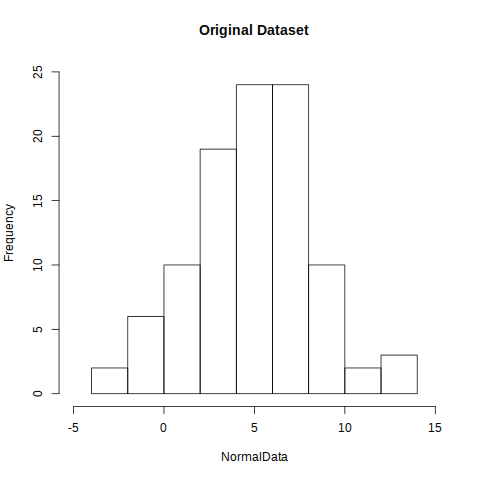
\includegraphics[width=\linewidth]{prob1a.png}

          The mean of \texttt{NormalData} is \num{4.996492}.

          The standard deviation of \texttt{NormalData} is \num{3.352686}.
        \item
          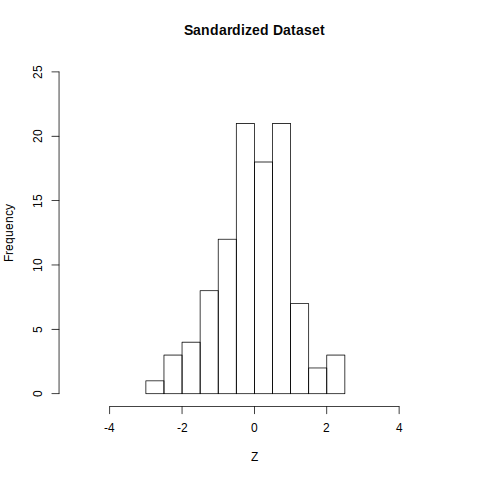
\includegraphics[width=\linewidth]{prob1b.png}

          The mean of \texttt{Z} is \num{-6.168026e-17}.

          The standard deviation of \texttt{Z} is 1.
        \item
          The transformation moved the data so that it is now centered at 0.
          The data is also more heavily weighted towards 0.
          The range of data is also smaller.
          The height appears to be just a touch smaller than before.
          The overall shape is still the same,
          it still appears to be normal.
      \end{enumerate}
    \item
      \begin{enumerate}
        \item
          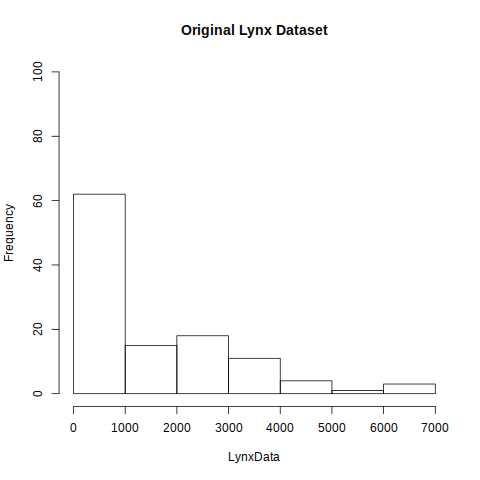
\includegraphics[width=\linewidth]{prob2a.png}

          The mean of LynxData is \num{1538.018}.

          The sd of LynxData is \num{1585.844}.

        \item
          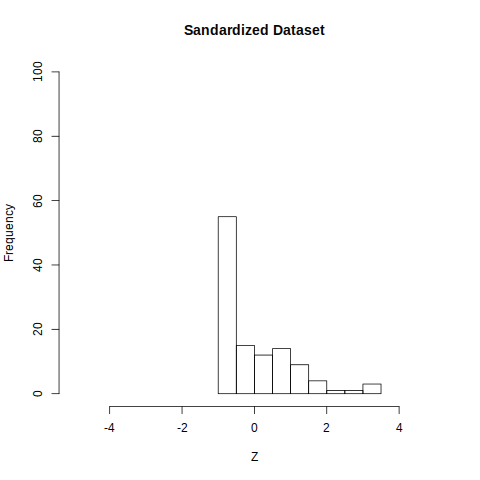
\includegraphics[width=\linewidth]{prob2b.png}

          The mean of Z is \num{4.221636e-17}.

          The sd of Z is \num{1}.

        \item
          The transformation moved the data so that it is now much closer to 0.
          The data is also more heavily weighted towards 0.
          The range of data is also smaller.
          The height appears to be just a touch smaller than before.
          The overall shape is still the same.
      \end{enumerate}
    \item
      \begin{enumerate}
        \item
          \begin{enumerate}
            \item
              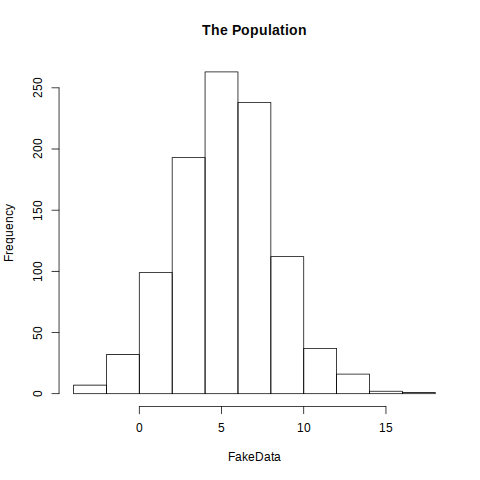
\includegraphics[width=\linewidth]{prob3a.png}

            \item
              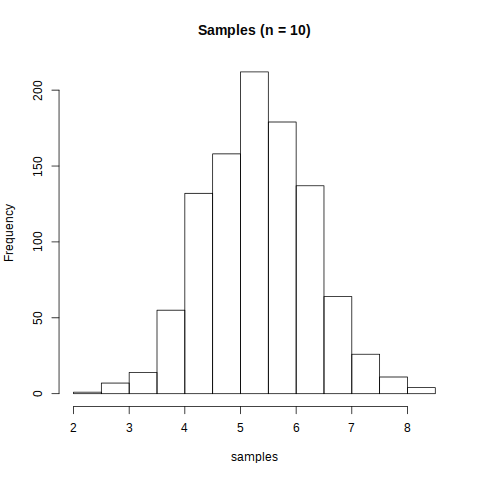
\includegraphics[width=\linewidth]{prob3a_ii.png}

              The mean for part ii is \num{4.798459}.

              The sd for part ii is \num{0.9308756}.
            \item
              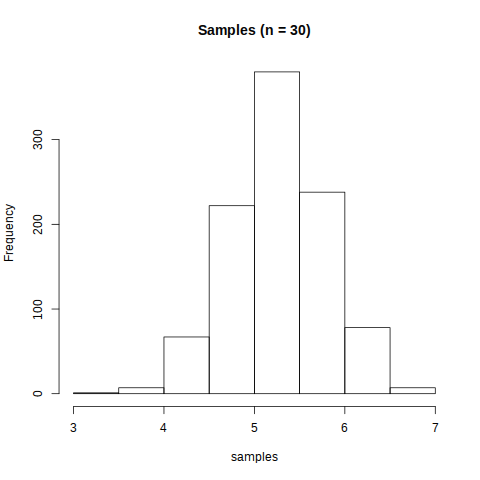
\includegraphics[width=\linewidth]{prob3a_iii.png}

              The mean for part iii is \num{4.794909}.

              The sd for part iii is \num{0.5519573}.
            \item
              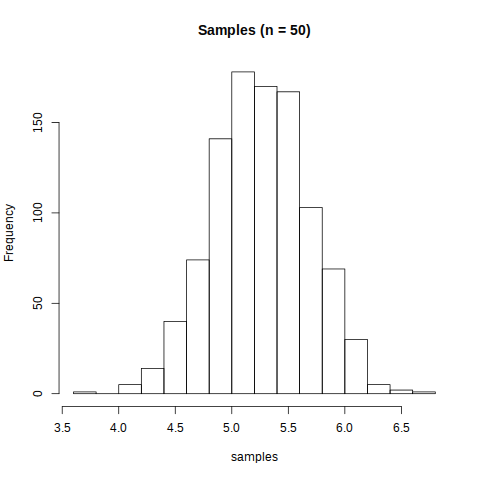
\includegraphics[width=\linewidth]{prob3a_iv.png}

              The mean for part iv is \num{4.781895}.

              The sd for part iv is \num{0.4373919}.
            \item
              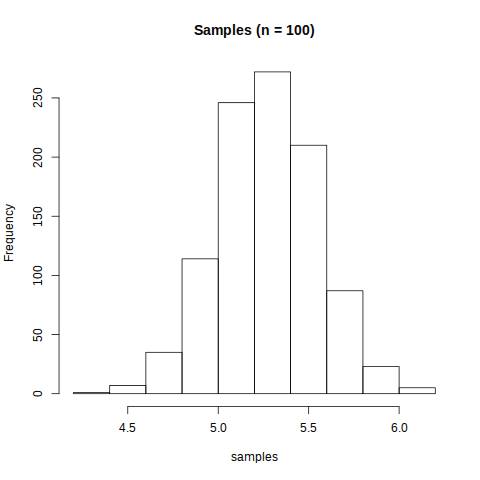
\includegraphics[width=\linewidth]{prob3a_v.png}

              The mean for part v is \num{4.772491}.

              The sd for part v is \num{0.2978722}.
          \end{enumerate}
        \item
          \begin{enumerate}
            \item
              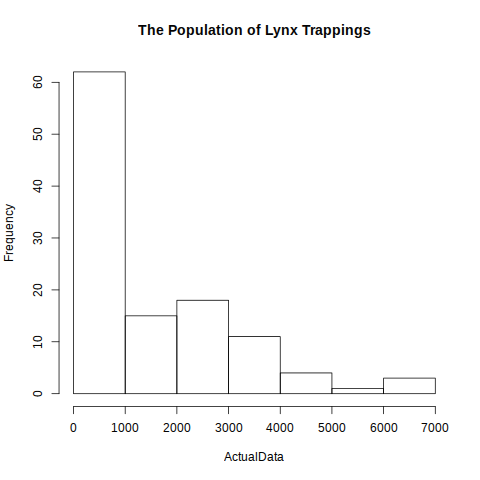
\includegraphics[width=\linewidth]{prob3b.png}

            \item
              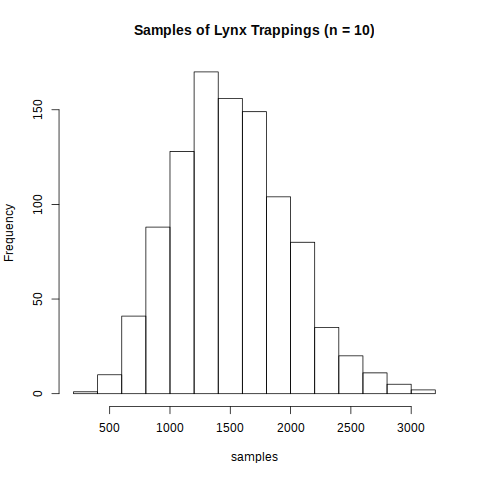
\includegraphics[width=\linewidth]{prob3b_ii.png}

              The mean for part ii is \num{1524.602}.

              The sd for part ii is \num{462.2495}.
            \item
              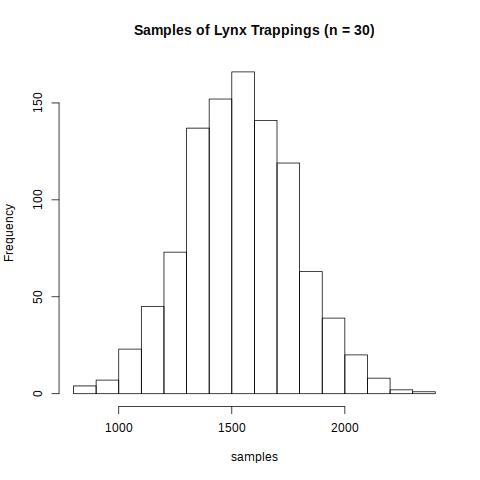
\includegraphics[width=\linewidth]{prob3b_iii.png}

              The mean for part iii is \num{1529.033}.

              The sd for part iii is \num{251.5058}.
            \item
              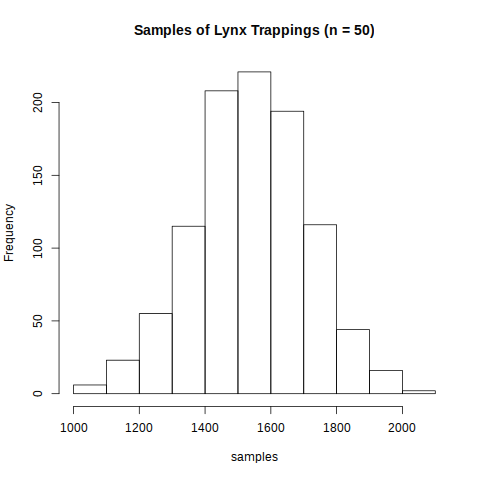
\includegraphics[width=\linewidth]{prob3b_iv.png}

              The mean for part iv is \num{1544.506}.

              The sd for part iv is \num{163.683}.
            \item
              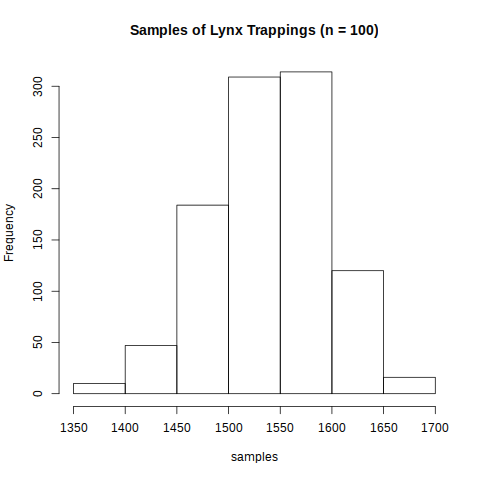
\includegraphics[width=\linewidth]{prob3b_v.png}

              The mean for part v is \num{1536.763}.

              The sd for part v is \num{55.27644}.
          \end{enumerate}
        \item
          The distributions in parts a and b are both approximately normal distributions.
          It appears that as $n$ increases, the range of values decreases, e.g.

      \end{enumerate}
  \end{enumerate}

  \begin{appendices}
    \section{R code}

        \subsection*{Problem 1}
            \rData{prob1.R}
            \subsubsection*{(a)}
                \rData{prob1a.R}
            \subsubsection*{(b)}
                \rData{prob1b.R}

        \subsection*{Problem 2}
            \rData{prob2.R}
            \subsubsection*{(a)}
                \rData{prob2a.R}
            \subsubsection*{(b)}
                \rData{prob2b.R}

        \subsection*{Problem 3}
            \rData{prob3.R}
            \subsubsection*{(a)}
                \rData{prob3a.R}
            \subsubsection*{(b)}
                \rData{prob3b.R}

\end{appendices}


\end{document}
